

\section{Automata and rational expressions \protect\\
\eee\ee on free monoids with weights in a field}
\label{sec:aut-fre-fld}%

Three instances of \tafkitv implement a weight semiring which is a 
\emph{field}:
\index{field}%
\code{vcsn-char-q}, \code{vcsn-char-r}, and \code{vcsn-char-f2}, 
for which the weight semiring is~$\Q$, $\R$, 
and~$\F_{2}=\Z/2\Z$ respectively (\cf \sbsct{taf-ins}).
In addition to all the functions of the preceding section which 
obviously apply, a function \Fct{reduce} is specific to those automata 
whose weight semiring is a field. 
It then easily allows to test the \emph{equivalence} of 
two automata or expressions.

\renewcommand{\theenumii}{\theenumi.\arabic{enumii}}

\begin{enumerate}

\item Operations on automata

\begin{enumerate}
\item \Fctaut{reduce}
\item \FctautD{are-equivalent}
\end{enumerate}

\item Operations on expressions

\begin{enumerate}
\item \FctexpD{are-equivalent-E}
\end{enumerate}

\end{enumerate}


\subsection{Operations on automata}
\label{ssc:ope-aut-fld}%

\subsubsection{\Fct{reduce}}

\begin{SwClCmd}
\begin{shell}
$ \kbd{vcsn reduce a.xml > b.xml}
$
\end{shell}%
\end{SwClCmd}%
\begin{SwClTxt}
    Computes from \Prm{a.xml} an equivalent 
    automaton of minimal dimension and writes the result in \Prm{b.xml}. 
\end{SwClTxt}%
\IndexFct{reduce}

\Prec \Prm{a.xml} is realtime.

\Comt Implements Sch\"utzenberger algorithm for reduction of 
representations (\cf \secti{aut-fre-fld-A}).

\Cave
\thi The reduction algorithm may well produce an automaton which will 
look more `complicated' than the original one, especially when the 
latter is already of minimal dimension.
\figur{red-bad} shows such an example.

\begin{figure}[ht]
    \centering
\includegraphics[scale=0.45]{figures/cc2q.ps}
\eee
\includegraphics[scale=0.45]{figures/cc2r.ps}
\caption{The quotient of \code{cc2.xml} and its `reduction'.}
\label{fig:red-bad}
\end{figure}


\thii
The computation of reduced representations implies the \emph{exact} 
resolution of  
linear systems of equations which becomes problematic when the 
dimension of the systems grows. 
The following example shows an error occurs when dealing with systems 
of dimension 32 (in~$\R$) ou 1024 (in~$\Q$): the number of states 
should be~$6$ in the first case, $11$~in the second.\footnote{%
   These data depend heavily on the examples, \emph{and also} on the machine on 
   which the examples are run.}

\begin{shell}
$ \kbd{vcsn-char-r power c1.xml 5 \bslash| reduce -  \bslash| data -}
States: 10
Transitions: 88
Initial states: 1
Final states: 1
$ \kbd{vcsn-char-q power c1.xml 10 \bslash| reduce -  \bslash| data -}
States: 25
Transitions: 444
Initial states: 1
Final states: 1
\end{shell}%


\subsubsection{\Fct{are-equivalent}}
\SetTwClPrm{\TwClOne}%

\begin{SwClCmd}
\begin{shell}
$ \kbd{vcsn -v are-equivalent a.xml b.xm }
Automata are not equivalent
\end{shell}%
\end{SwClCmd}%
\begin{SwClTxt}
    Tells whether or not the automata  \Prm{a.xml} and \Prm{b.xml} 
    realize the same series. 
\end{SwClTxt}%
\IndexFct{are-equivalent}

\Prec no precondition.

\Spec
\Fctq{are-equivalent}{{a.xml},{b.xml}} =\\  
\e\Fctq{is-empty}{\Fctq{reduce}{\Fctq{sum}{\Fctq{standardize}{\Fctq{realtime}{a.xml}},\\
\eee \eee\ee\e 
\Fctq{left-mult}{\Fctq{standardize}{\Fctq{realtime}{b.xml}},-1}}}}

\longonly{%
\begin{ComVd}{110709}
In \tafkitv,  what is really implemented is:
	
\noindent 	
\Fctq{are-equivalent}{{a.xml},{b.xml}} =\\  
\e\Fctq{is-useless}{\Fctq{reduce}{\Fctq{sum}{\Fctq{standardize}{\Fctq{realtime}{a.xml}},\\
\eee\eee\ee\ee
\Fctq{left-mult}{\Fctq{standardize}{\Fctq{realtime}{b.xml}},-1}}}}
	
\noindent
but it is equivalent.
\end{ComVd}%
}%


\subsection{Operations on expressions}


\subsubsection{\Fct{are-equivalent-E}}
\SetTwClPrm{\TwClThree}%

\begin{SwClCmd}
\begin{shell}
$ \kbd{vcsn -v -ixml are-equivalent-E e.xml f.xml}
Expressions are equivalent
\end{shell}%
\end{SwClCmd}%
\begin{SwClTxt}
    Tells whether or not the expressions  \Prm{e.xml} and \Prm{f.xml} 
    denote the same language. 
\end{SwClTxt}%
\IndexFct{are-equivalent-E}%


\Spec
\Fctq{are-equivalent-E}{{e.xml},{f.xml}} =
\Fctq{are-equivalent}{\Fctq{standard}{e.xml},\Fctq{standard}{f.xml}}

\Cave
The specifications for the input format of rational expressions apply 
for this function.
For instance, the alphabet must be specified if the expressions are 
given as strings.

\Exam

\shortonly{\medskipneg}  
\begin{shell}
$ \kbd{vcsn-char-q -aab -v are-equivalent-E 'b*((\{2\}a).b*)*' '((\{2\}a)*b)*(\{2\}a)*'}
Expressions are equivalent
\end{shell}%
   

\SetTwClPrm{\TwClOne}%
%%%%%%%%%%%%%%%%%%%%%%%%
\endinput
